\documentclass{standalone}
\usepackage{tikz}
\usetikzlibrary{positioning}

\begin{document}

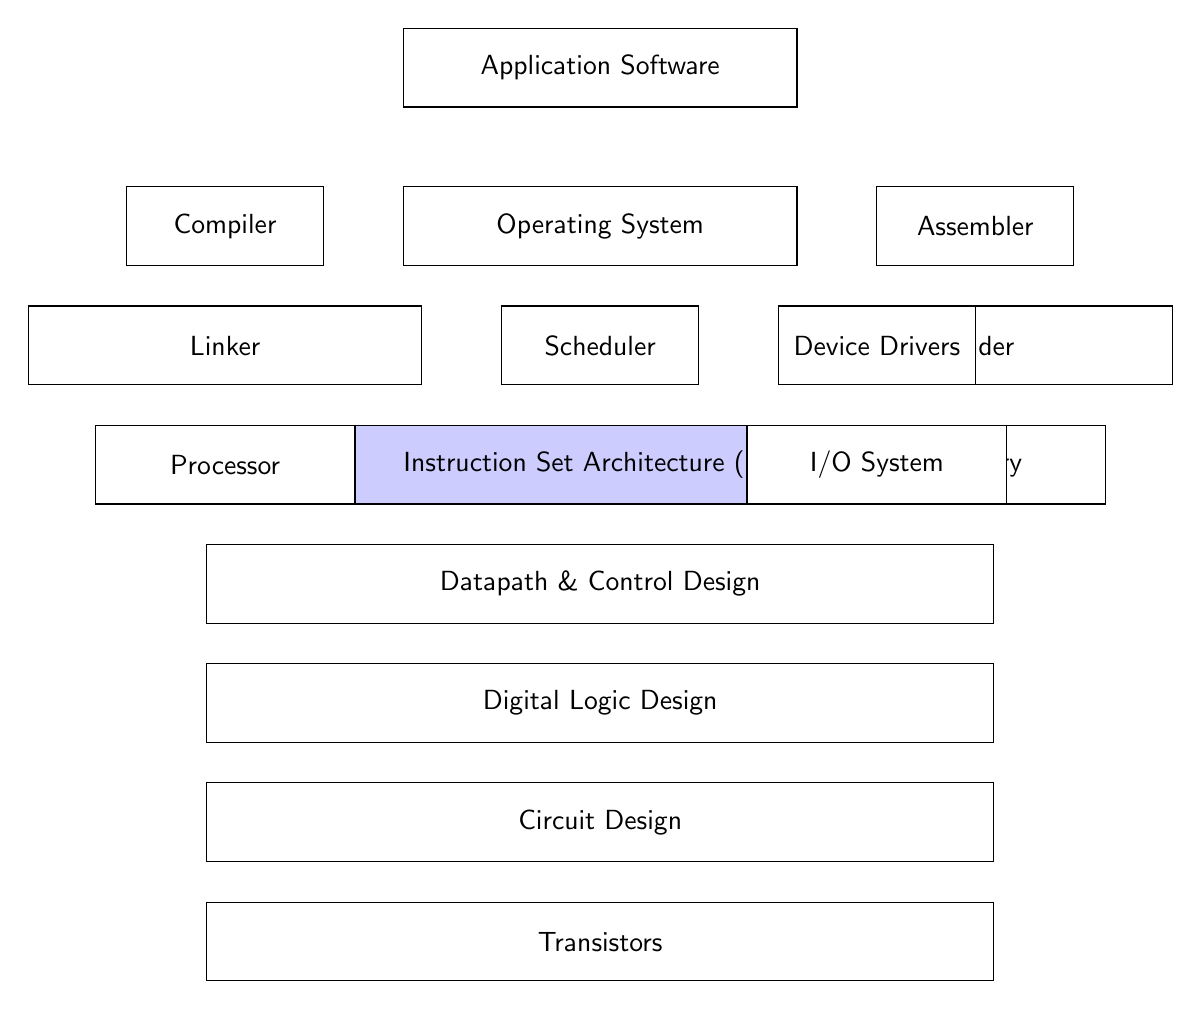
\begin{tikzpicture}[
  font=\sffamily,
  box/.style={draw, fill=white, minimum width=5cm, minimum height=1cm, align=center},
  level 1/.style={sibling distance=5cm},
  level 2/.style={sibling distance=3cm}
]

% Application Software
\node[box] (app) {Application Software};

% Compiler, Assembler
\node[box, below left=of app, minimum width=2.5cm] (compiler) {Compiler};
\node[box, below right=of app, minimum width=2.5cm] (assembler) {Assembler};

% Operating System
\node[box, below=1cm of app] (os) {Operating System};

% Linker, Loader, Scheduler, Device Drivers
\node[box, below=0.5cm of compiler] (linker) {Linker};
\node[box, below=0.5cm of assembler] (loader) {Loader};
\node[box, below=0.5cm of os, minimum width=2.5cm] (scheduler) {Scheduler};
\node[box, right=of scheduler, minimum width=2.5cm] (drivers) {Device Drivers};

% Instruction Set Architecture (ISA)
\node[box, below=0.5cm of scheduler, minimum width=10cm, fill=blue!20] (isa) {Instruction Set Architecture (ISA)};

% Processor, Memory, I/O System
\node[box, below=0.5cm of linker, minimum width=3.3cm] (processor) {Processor};
\node[box, below=0.5cm of loader, minimum width=3.3cm] (memory) {Memory};
\node[box, below=0.5cm of drivers, minimum width=3.3cm] (io) {I/O System};

% Datapath & Control Design
\node[box, below=0.5cm of isa, minimum width=10cm] (datapath) {Datapath \& Control Design};

% Digital Logic Design
\node[box, below=0.5cm of datapath, minimum width=10cm] (logic) {Digital Logic Design};

% Circuit Design
\node[box, below=0.5cm of logic, minimum width=10cm] (circuit) {Circuit Design};

% Transistors
\node[box, below=0.5cm of circuit, minimum width=10cm] (transistors) {Transistors};

\end{tikzpicture}

\end{document}
